\chapter{Eksperymenty dla licencji Duolingo Super}
\label{chap:experiments}

\section{Środowisko i metodologia}

Eksperymenty wykonano na komputerze z procesorem Intel Core i5-14600KF (12 rdzeni ograniczone przez konfigurację WSL2, taktowanie 3,49~GHz) oraz 16~GB pamięci RAM. System operacyjny stanowił Ubuntu~24.04~LTS uruchomiony w środowisku WSL2. Implementacja algorytmów powstała w języku Python~3.13; wykorzystano biblioteki NumPy, NetworkX, a także PuLP jako interfejs do solverów ILP. Każdy pomiar obejmował wyłącznie czas obliczeń, pomijając koszt przygotowania instancji oraz operacje wejścia/wyjścia.

Analiza objęła dwa zestawy danych: syntetyczne grafy losowe, bezskalowe oraz małoświatowe o liczebności od 50 do 450 wierzchołków, a także grafy ego z serwisu Facebook o liczebności od 53 do 1035 wierzchołków. Dla każdej instancji uruchamiano wszystkie algorytmy z limitem czasu wynoszącym 60 sekund, a przekroczenie tego limitu oznaczano jako timeout i wyłączano z dalszych obliczeń. Na grafach syntetycznych odnotowano 10 timeoutów dla algorytmu mrówkowego oraz solvera ILP, natomiast na grafach rzeczywistych odpowiednio 8, 18 i 6 przypadków dla algorytmu mrówkowego, solvera ILP oraz przeszukiwania tabu. Wszystkie pozostałe uruchomienia zakończyły się sukcesem.

W przypadku grafów syntetycznych dla każdego rozmiaru generowano trzy niezależne instancje, a następnie wykonywano po dwa uruchomienia algorytmów na każdej z nich. Analiza sieci ego Facebooka obejmowała po jednym grafie na rozmiar oraz dwa powtórzenia dla każdej pary (graf, algorytm), co pozwoliło oszacować zmienność wyników przy zachowaniu rozsądnego budżetu obliczeniowego.
W każdej próbie zapisano całkowity koszt licencji, czas wykonania oraz koszt w przeliczeniu na wierzchołek. Wyniki agregowano przez średnią. Spójność różnic między algorytmami oceniono przy użyciu testów Friedmana, gdzie $\chi^2_F$ to wartość statystyki testu Friedmana oraz $p$ to poziom istotności, a następnie następujących po nich porównań post-hoc metodą Nemenyi'ego. Na syntetycznym benchmarku otrzymano statystyki $\chi^2_F = 577{,}93$ dla czasu oraz $\chi^2_F = 518{,}01$ dla kosztu na węzeł ($p < 10^{-100}$ w obu przypadkach), co uzasadnia szczegółowe porównania par algorytmów.

\section{Duolingo Super na grafach syntetycznych}

\subsection{Statystyki zbiorcze}
Tabela~\ref{tab:duo-synth-summary} zestawia średnie wartości kosztu na węzeł oraz czasu dla licencji Duolingo Super. \textbf{Solver~ILP} pozostaje najlepszym punktem odniesienia jakościowego (średni koszt na węzeł 0,445), lecz przydaje się jedynie dla mniejszych instancji. Posiada tyle samo timeoutów co \textbf{Algorytm mrówkowy}. Wśród metaheurystyk najniższy koszt na węzeł osiąga właśnie \textbf{Algorytm mrówkowy} (0,506), natomiast \textbf{Przeszukiwanie tabu} zapewnia najlepszy kompromis kosztu na węzeł i czasu w grupie metod przybliżonych. \textbf{Algorytm zachłanny} i \textbf{Algorytm losowy} działają prawie natychmiast, ale tylko pierwszy z nich zachowuje akceptowalny koszt na węzeł (0,548), podczas gdy losowy baseline pozostaje wyraźnie gorszy jakościowo.

\begin{table}[H]
  \centering
  \caption{Średnie wartości kosztu na węzeł i czasu dla licencji Duolingo Super na grafach syntetycznych.}
  \label{tab:duo-synth-summary}
  \begin{tabular}{lrrr}
    \toprule
    \textbf{Algorytm}     & \textbf{Średni koszt/węzeł} & \textbf{Średni koszt} & \textbf{Średni czas [s]} \\
    \midrule
    Solver ILP            & 0.445                       & 73.83                 & 2.492                    \\
    Algorytm mrówkowy     & 0.506                       & 83.58                 & 5.124                    \\
    Przeszukiwanie tabu   & 0.500                       & 117.80                & 3.298                    \\
    Algorytm genetyczny   & 0.515                       & 118.36                & 1.222                    \\
    Wyżarzanie symulowane & 0.531                       & 120.90                & 0.975                    \\
    Zbiór dominujący      & 0.542                       & 119.97                & 0.017                    \\
    Algorytm zachłanny    & 0.548                       & 121.94                & 0.001                    \\
    Algorytm losowy       & 0.799                       & 179.90                & 0.001                    \\
    \bottomrule
  \end{tabular}
\end{table}


\subsection{Porównanie algorytmów na grafach syntetycznych}

Rysunki~\ref{fig:duo-synth-cost-random}--\ref{fig:duo-synth-cost-small-world} pokazują, że algorytmy dla licencji Duolingo Super osiągają wyniki porównywalne z solverem ILP w przypadku grafów losowych i małoświatowych. Natomiast w przypadku grafów bezskalowych wyniki są zauważalnie gorsze.


\begin{figure}[H]
  \centering
  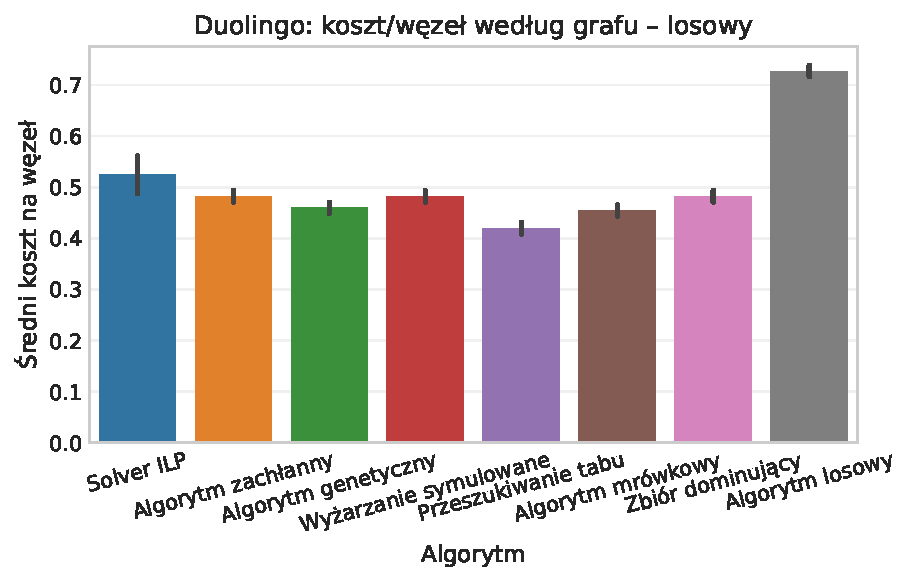
\includegraphics[width=0.65\linewidth]{assets/figures/benchmark/synthetic/duolingo_cost_per_node_by_graph_random.pdf}
  \caption{Koszt na węzeł w zależności od struktury grafu losowej.}
  \label{fig:duo-synth-cost-random}
\end{figure}

\begin{figure}[H]
  \centering
  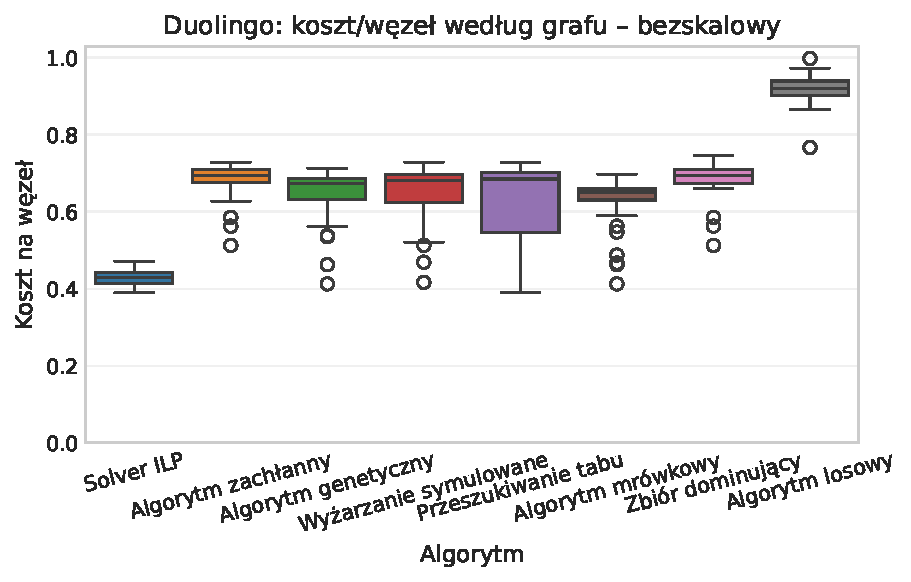
\includegraphics[width=0.65\linewidth]{assets/figures/benchmark/synthetic/duolingo_cost_per_node_by_graph_scale_free.pdf}
  \caption{Koszt na węzeł w zależności od struktury grafu bezskalowej.}
  \label{fig:duo-synth-cost-scale-free}
\end{figure}

\begin{figure}[H]
  \centering
  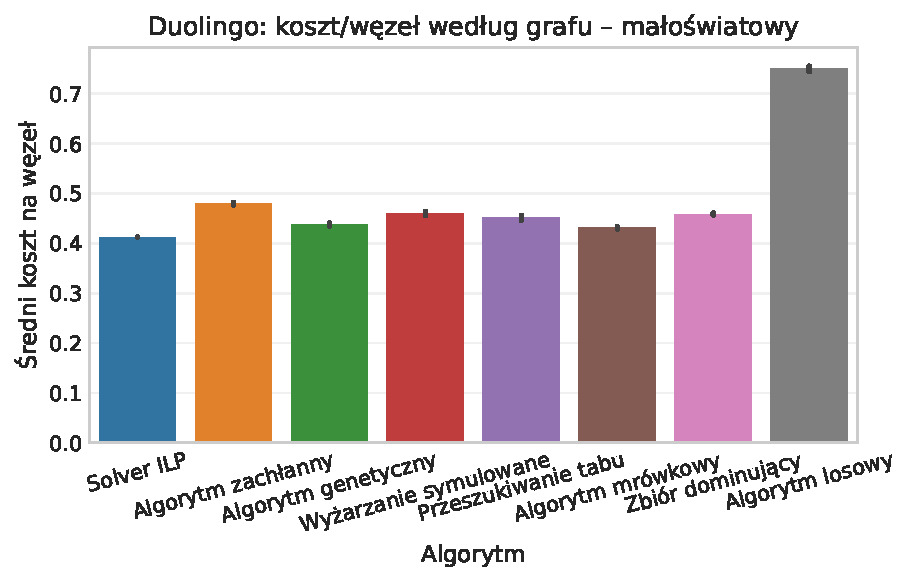
\includegraphics[width=0.65\linewidth]{assets/figures/benchmark/synthetic/duolingo_cost_per_node_by_graph_small_world.pdf}
  \caption{Koszt na węzeł w zależności od struktury grafu małoświatowej.}
  \label{fig:duo-synth-cost-small-world}
\end{figure}

Podobne obserwacje dotyczą czasów wykonania, jak ilustrują rysunki~\ref{fig:duo-synth-time-random}--\ref{fig:duo-synth-time-small-world}. Czasy działania algorytmów są zbliżone dla różnych typów grafów, z wyjątkiem solvera ILP, który średnio działa szybciej na grafach bezskalowych, oraz przeszukiwania tabu, które działa na nich dłużej. Pozostałe algorytmy wykazują porównywalne czasy działania niezależnie od struktury grafu. Tabela~\ref{tab:duo-synth-summary-times} podsumowuje średnie czasów i kosztów na węzeł dla różnych typów grafów.

\begin{figure}[H]
  \centering
  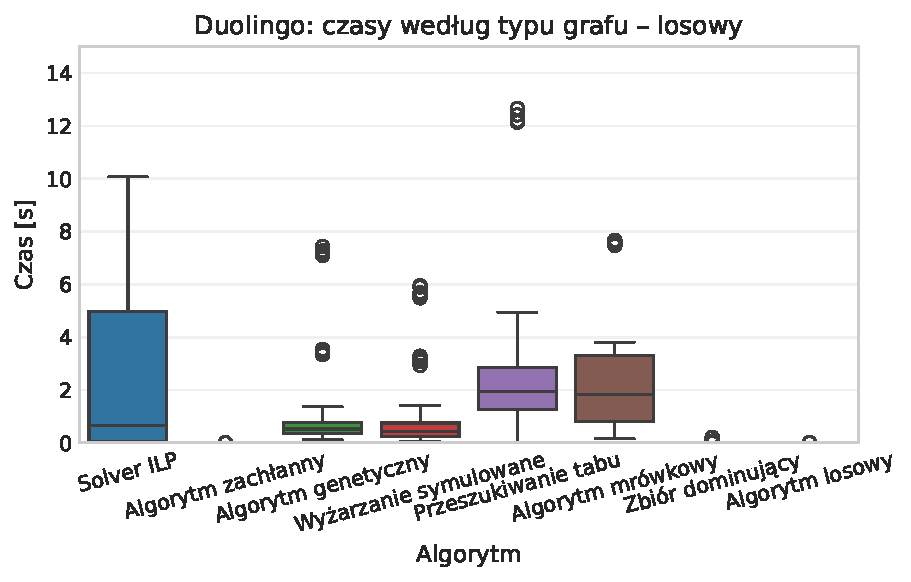
\includegraphics[width=0.65\linewidth]{assets/figures/benchmark/synthetic/duolingo_time_by_graph_random.pdf}
  \caption{Czas wykonania w zależności od struktury grafu losowej.}
  \label{fig:duo-synth-time-random}
\end{figure}

\begin{figure}[H]
  \centering
  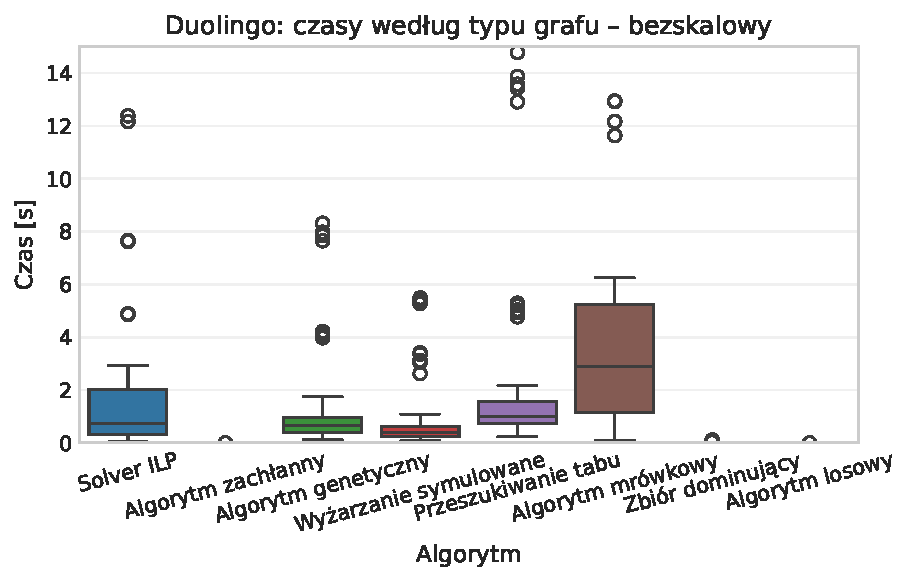
\includegraphics[width=0.65\linewidth]{assets/figures/benchmark/synthetic/duolingo_time_by_graph_scale_free.pdf}
  \caption{Czas wykonania w zależności od struktury grafu bezskalowej.}
  \label{fig:duo-synth-time-scale-free}
\end{figure}

\begin{figure}[H]
  \centering
  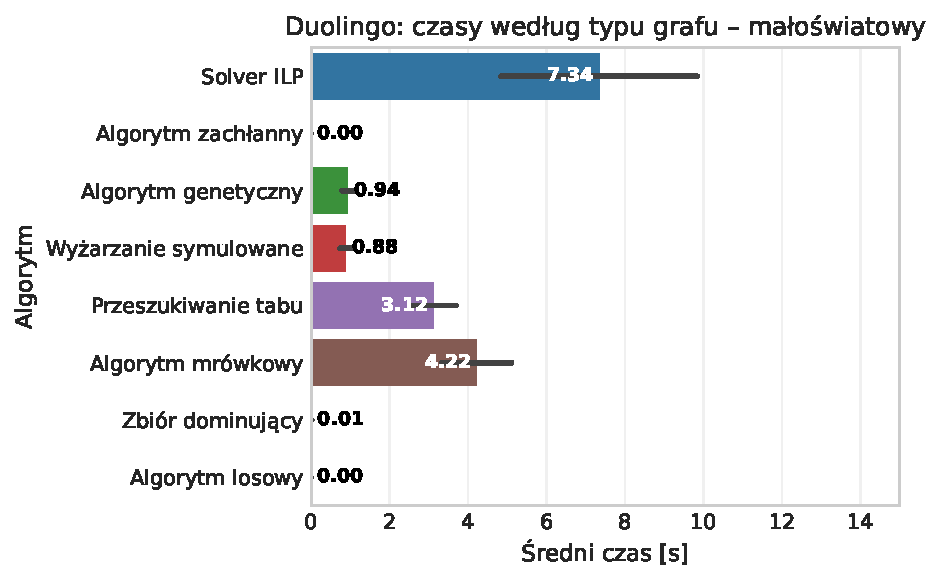
\includegraphics[width=0.65\linewidth]{assets/figures/benchmark/synthetic/duolingo_time_by_graph_small_world.pdf}
  \caption{Czas wykonania w zależności od struktury grafu małoświatowej.}
  \label{fig:duo-synth-time-small-world}
\end{figure}

\begin{table}[H]
  \centering
  \caption{Średnie koszty i czasy na węzeł dla różnych typów grafów (Duolingo Super i dominowanie rzymskie).}
  \label{tab:duo-synth-summary-times}
  \begin{tabular}{lcccc}
    \toprule
    \textbf{Licencja}    & \textbf{Typ grafu} & \textbf{Śr. koszt/węzeł} & \textbf{Śr. czas [s]} \\
    \midrule
    Duolingo Super       & Bezskalowy         & 0.661                    & 1.655                 \\
    Duolingo Super       & Losowy             & 0.502                    & 1.598                 \\
    Duolingo Super       & Małoświatowy       & 0.495                    & 1.346                 \\
    Dominowanie rzymskie & Bezskalowy         & 0.490                    & 0.913                 \\
    Dominowanie rzymskie & Losowy             & 0.344                    & 0.815                 \\
    Dominowanie rzymskie & Małoświatowy       & 0.409                    & 1.544                 \\
    \bottomrule
  \end{tabular}
\end{table}

Z powyższych danych wynika, że struktura grafu ma istotny wpływ zarówno na koszty, jak i na czasy działania algorytmów. Licencja Duolingo Super radzi sobie najgorzej w przypadku grafów bezskalowych. Z kolei licencja dominowania rzymskiego osiąga najgorsze wyniki dla grafów małoświatowych, podczas gdy w przypadku grafów bezskalowych wypada najlepiej.

\section{Duolingo Super na grafach rzeczywistych}
W analizie grafów ego z serwisu Facebook pominięto obserwacje, w których solver ILP nie zakończył pracy przed limitem czasu (18 przypadków). Dodatkowo odnotowano 8 timeoutów algorytmu mrówkowego i 6 przypadków w przeszukiwaniu tabu; pozostałe uruchomienia zakończyły się sukcesem.

\begin{table}[H]
  \centering
  \caption{Statystyki kosztu i czasu dla licencji Duolingo Super na grafach rzeczywistych.}
  \label{tab:duo-real-alg}
  \begin{tabular}{lrrr}
    \toprule
    \textbf{Algorytm}     & \textbf{Średni koszt} & \textbf{Śr. koszt/węzeł} & \textbf{Śr. czas [s]} \\
    \midrule
    Algorytm mrówkowy     & 83.58                 & 0.506                    & 5.124                 \\
    Zbiór dominujący      & 119.97                & 0.542                    & 0.017                 \\
    Algorytm genetyczny   & 118.36                & 0.515                    & 1.222                 \\
    Algorytm zachłanny    & 121.94                & 0.548                    & 0.001                 \\
    Algorytm losowy       & 179.90                & 0.799                    & 0.001                 \\
    Wyżarzanie symulowane & 120.90                & 0.531                    & 0.975                 \\
    Przeszukiwanie tabu   & 117.80                & 0.500                    & 3.298                 \\
    \bottomrule
  \end{tabular}
\end{table}
Tabela~\ref{tab:duo-real-alg} pokazuje, że zarówno przeszukiwanie tabu, jak i algorytm mrówkowy zachowują przewagę kosztową nad heurystykami losowymi i zachłannymi, choć okupują ją dłuższym czasem działania.

\subsection{Skalowanie i jakość}

Rysunek~\ref{fig:duo-real-size} pokazuje, że wraz ze wzrostem liczby wierzchołków koszt na węzeł rośnie umiarkowanie, przy czym przeszukiwanie tabu utrzymuje najniższe wartości, a algorytm mrówkowy plasuje się tuż za nim. Czasy działania wszystkich metod mieszczą się w przedziale do kilku sekund i rosną łagodnie wraz z rozmiarem grafu; algorytm zachłanny nadal pozostaje niemal natychmiastowy i stanowi dobry punkt startowy dla metaheurystyk. Dodatkowo tabela~\ref{tab:duo-real-size-table} zbiera średnie wartości (TabuSearch) dla kolejnych rozmiarów sieci ego i pokazuje, że koszt na węzeł utrzymuje się w przedziale 1{,}8--2{,}5 przy czasie rosnącym od ułamka sekundy do około 5{,}5~s dla największych grafów.

\begin{figure}[H]
  \centering
  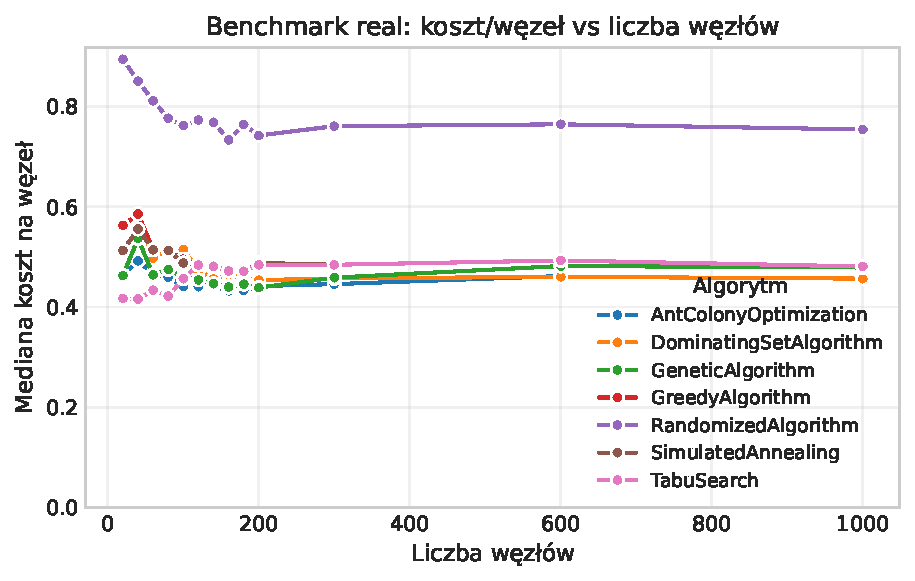
\includegraphics[width=0.48\linewidth]{assets/figures/benchmark/real/cost_per_node_vs_nodes.pdf}
  \hfill
  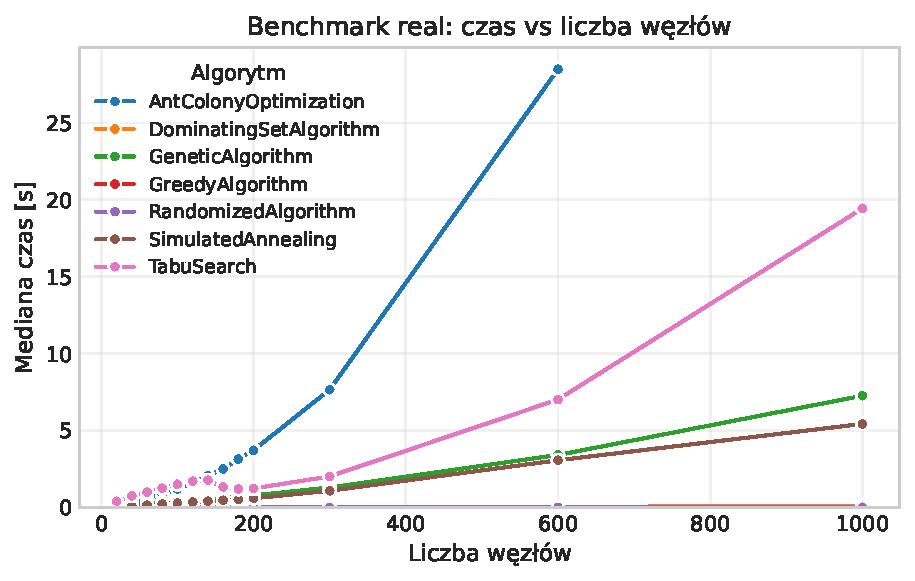
\includegraphics[width=0.48\linewidth]{assets/figures/benchmark/real/time_vs_nodes.pdf}
  \caption{Koszt na węzeł i czas wykonania licencji Duolingo Super w funkcji liczby wierzchołków (grafy ego Facebook).}
  \label{fig:duo-real-size}
\end{figure}

\begin{table}[H]
  \centering
  \caption{Średni koszt na węzeł i czas (przeszukiwanie tabu) względem liczby wierzchołków w sieciach ego Facebook.}
  \label{tab:duo-real-size-table}
  \begin{tabular}{lrr}
    \toprule
    \textbf{Liczba wierzchołków} & \textbf{Śr. koszt/węzeł} & \textbf{Śr. czas [ms]} \\
    \midrule
    53                           & 6.175                    & 2161.349               \\
    62                           & 5.175                    & 3141.926               \\
    151                          & 5.297                    & 6825.722               \\
    169                          & 5.499                    & 8726.145               \\
    225                          & 5.704                    & 12324.041              \\
    334                          & 7.843                    & 32705.396              \\
    535                          & 7.400                    & 58557.464              \\
    \bottomrule
  \end{tabular}
\end{table}


\section{Porównanie z dominowaniem rzymskim}

Porównania z dominowaniem rzymskim ograniczono do wspólnych instancji i algorytmów. Rysunki~\ref{fig:duo-roman-cost}--\ref{fig:duo-roman-license} zestawiają różnice w kosztach, czasach i strukturze licencji, a tabela~\ref{tab:duo-roman-graph} gromadzi średnie według typu grafu syntetycznego.

\begin{table}[H]
  \centering
  \caption{Średnie czasu i kosztu na węzeł według typu grafu (wspólne instancje).}
  \label{tab:duo-roman-graph}
  \begin{tabular}{lcccc}
    \toprule
    \multirow{2}{*}{\textbf{Typ grafu}} & \multicolumn{2}{c}{\textbf{Duolingo Super}} & \multicolumn{2}{c}{\textbf{Dominowanie rzymskie}}                                            \\
                                        & \textbf{Czas [s]}                           & \textbf{Koszt/węzeł}                              & \textbf{Czas [s]} & \textbf{Koszt/węzeł} \\
    \midrule
    Losowy                              & 1.598                                       & 0.502                                             & 0.815             & 0.344                \\
    Bezskalowy                          & 1.655                                       & 0.661                                             & 0.913             & 0.490                \\
    Małoświatowy                        & 1.346                                       & 0.495                                             & 1.544             & 0.409                \\
    \bottomrule
  \end{tabular}
\end{table}

Dominowanie rzymskie zapewnia niższy koszt na węzeł we wszystkich porównywanych rodzinach grafów. Największa różnica dotyczy struktur losowych, gdzie przewaga wynosi ok.~0,16 punktu (32\%). W sieciach bezskalowych różnica maleje do 0,17, natomiast w małoświatowych do 0,09. Czasy wykonania są porównywalne, przy lekkiej przewadze Duolingo Super w grafach małoświatowych, ale dominowanie rzymskie jest szybsze w grafach losowych i bezskalowych. Rysunek~\ref{fig:duo-roman-cost} ilustruje te obserwacje dla pełnego rozkładu, a rysunek~\ref{fig:duo-roman-time} prezentuje analogiczne dane czasowe. Warto zauważyć, że wyższe koszty na węzeł w przypadku Duolingo Super wynikają z ograniczeń w opłacalności licencji grupowych. Licencja grupowa jest około 2,1 razy droższa od indywidualnej, co oznacza, że opłaca się ją tworzyć dopiero dla grup liczących co najmniej trzy osoby (właściciel i dwóch sąsiadów). W efekcie liczba licencji indywidualnych w Duolingo Super jest większa, co przekłada się na wyższy średni koszt na węzeł w porównaniu do dominowania rzymskiego.

\begin{figure}[H]
  \centering
  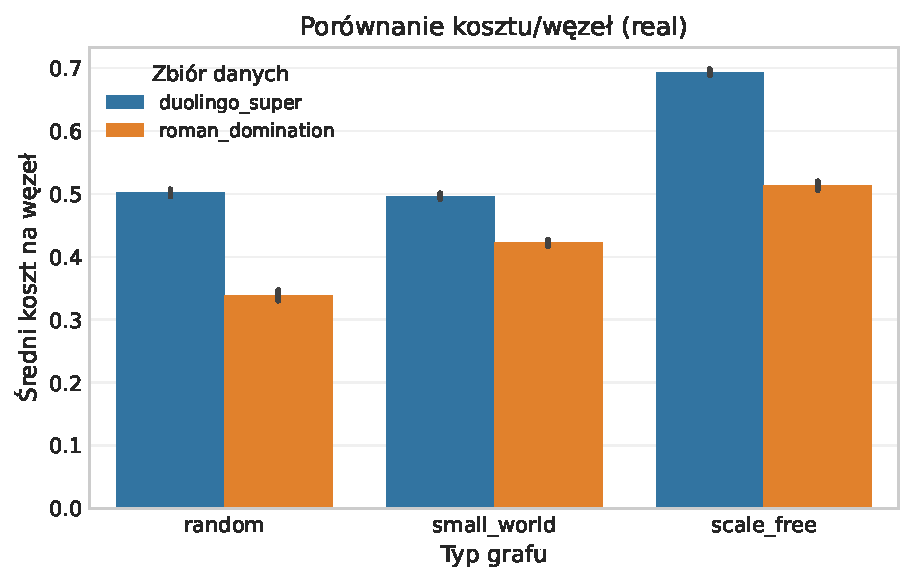
\includegraphics[width=0.6\linewidth]{assets/figures/benchmark/real/duo_vs_roman_cost_per_node_by_graph.pdf}
  \caption{Koszt na węzeł według typu grafu: porównanie licencji Duolingo Super i dominowania rzymskiego.}
  \label{fig:duo-roman-cost}
\end{figure}

\begin{figure}[H]
  \centering
  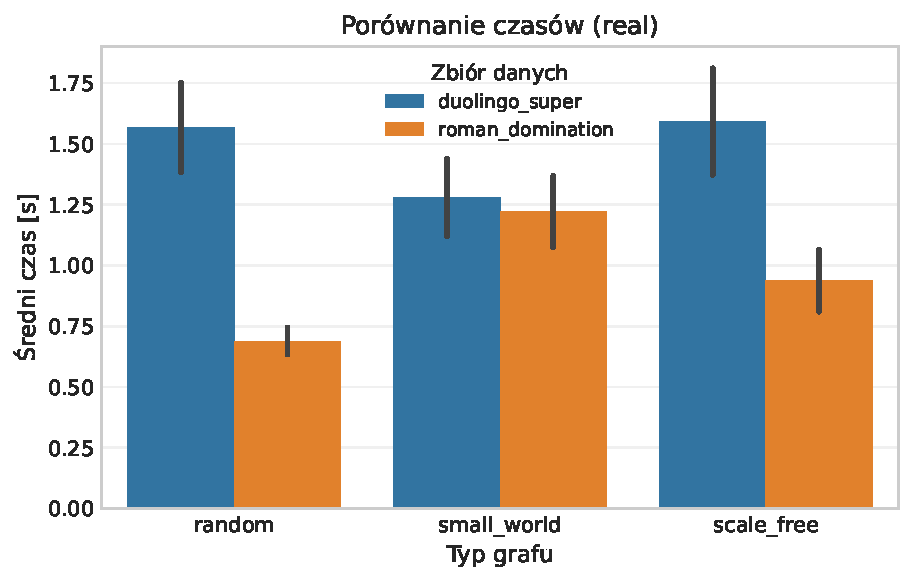
\includegraphics[width=0.6\linewidth]{assets/figures/benchmark/real/duo_vs_roman_time_by_graph.pdf}
  \caption{Czas wykonania według typu grafu: porównanie licencji Duolingo Super i dominowania rzymskiego.}
  \label{fig:duo-roman-time}
\end{figure}

Rysunek~\ref{fig:duo-roman-license} pokazuje, że dominowanie rzymskie charakteryzuje się wyższym stosunkiem licencji grupowych do indywidualnych w porównaniu do Duolingo Super. W przypadku dominowania rzymskiego stosunek ten wynosi około 1,15:1, podczas gdy dla Duolingo Super jest to około 0,88:1.

Różnica ta wynika z faktu, że dominowanie rzymskie nie posiada ograniczenia maksymalnej pojemności grupy licencyjnej. W przypadku Duolingo Super, gdy grupa osiąga maksymalną pojemność, dodatkowi użytkownicy, którzy mogliby do niej należeć, są zmuszeni do zakupu licencji indywidualnych. W pełnym zbiorze danych, obejmującym trzy typy grafów syntetycznych, zaobserwowano 137690 licencji w Duolingo Super, z czego 73176 (53,15\%) to licencje indywidualne. W przypadku dominowania rzymskiego, dzięki braku ograniczeń pojemności grup, liczba licencji indywidualnych jest proporcjonalnie niższa.

\begin{figure}[H]
  \centering
  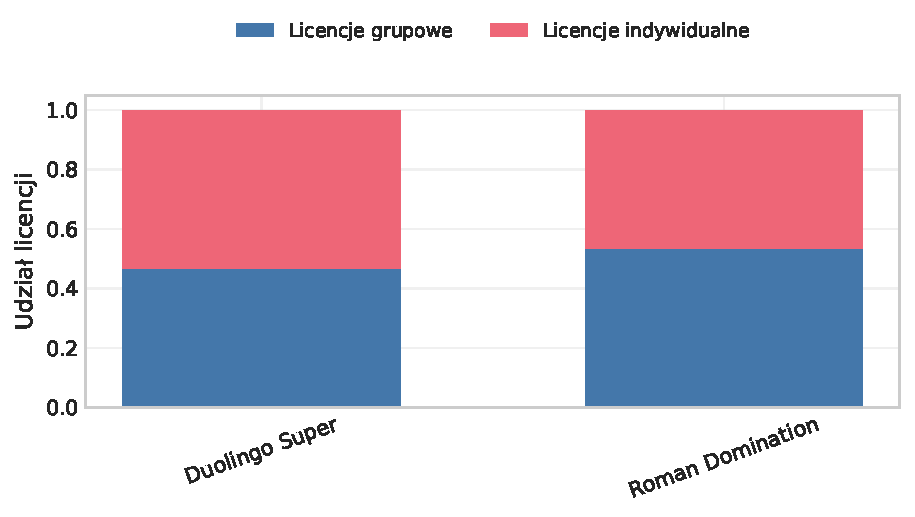
\includegraphics[width=0.6\linewidth]{assets/figures/benchmark/synthetic/license_mix_duo_vs_roman.pdf}
  \caption{Struktura wykorzystania licencji: porównanie licencji Duolingo Super i dominowania rzymskiego.}
  \label{fig:duo-roman-license}
\end{figure}

\section{Wnioski}

Analiza potwierdza dużą stabilność wyników Duolingo Super: metaheurystyki utrzymują przewagę jakości nad prostymi heurystykami niezależnie od rozmiaru i struktury grafu, a \textbf{Algorytm mrówkowy} oraz \textbf{Przeszukiwanie tabu} stanowią najbardziej konkurencyjną parę. Równocześnie dominowanie rzymskie pozostaje trudne do pobicia pod względem kosztu na węzeł, głównie dzięki większemu wykorzystaniu licencji grupowych i niższemu mnożnikowi kosztów jednostkowych.
